We were able to measure the prefetch size read by the system during a sequential 
read. In Linux, there is a readahead algorithm that fetches a certain number of 
pages from disk given the read behavior. The set of pages in the cache fetched by 
the algorithm is called the readahead window. In a normal sequential read, the 
readahead algorithm starts with an initial read size based on the first read and in
subsequent requests grows the readahead window until it reaches the maximum size. 
The readahead algorithm marks a page at the lookahead index. When the application 
references this page, the algorithm grows the readahead window and asynchronously 
fetches the next set of pages from disk.\cite{wu2010sequential}\cite{wu2007linux} 
The maximum window is determined by 
parameters in the kernel code, but it is typically 32 pages. In our system, we have
4KB pages so we expect the readahead size to grow exponentially and then plateau at
the maximum window size of 128KB. We expect the same for our virtual machine, which 
has the same readahead algorithm and page size since it uses the same kernel.

\begin{figure}[t!]
	\begin{algorithmic}
		\STATE open $file$
		\STATE clear cache
		\FOR{$i = $0 \TO $MAX\_READS$}
		\STATE start\_timer
		\STATE Read READ\_SIZE bytes
		\STATE end\_timer and save the result
		\STATE Wait 100ms
		\ENDFOR
		\STATE close $file$
		\STATE report recorded times
	\end{algorithmic}
	\caption{Pseudocode for measuring prefetch size}
	\label{fig:p2_code}
\end{figure}

\begin{figure}[hb!]
	\begin{subfigure}[t]{0.5\textwidth}
	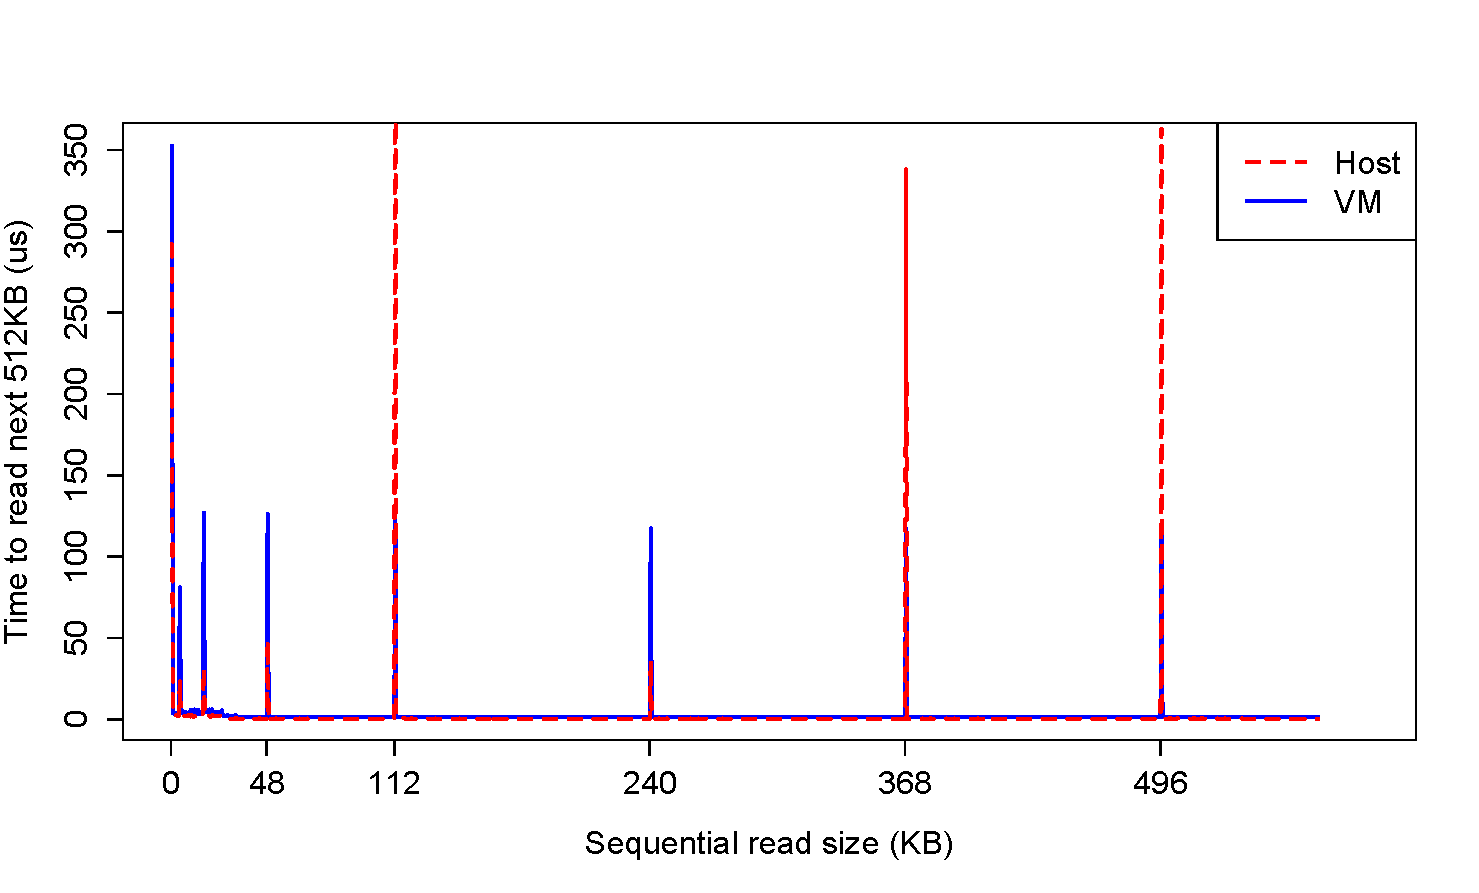
\includegraphics[width=\textwidth]{./figures/p2_big.pdf}
	\caption{A broad view of latency versus number of read bytes}
	\label{fig:p2_graph_big}
	\end{subfigure}
	
	\begin{subfigure}[t]{0.5\textwidth}
	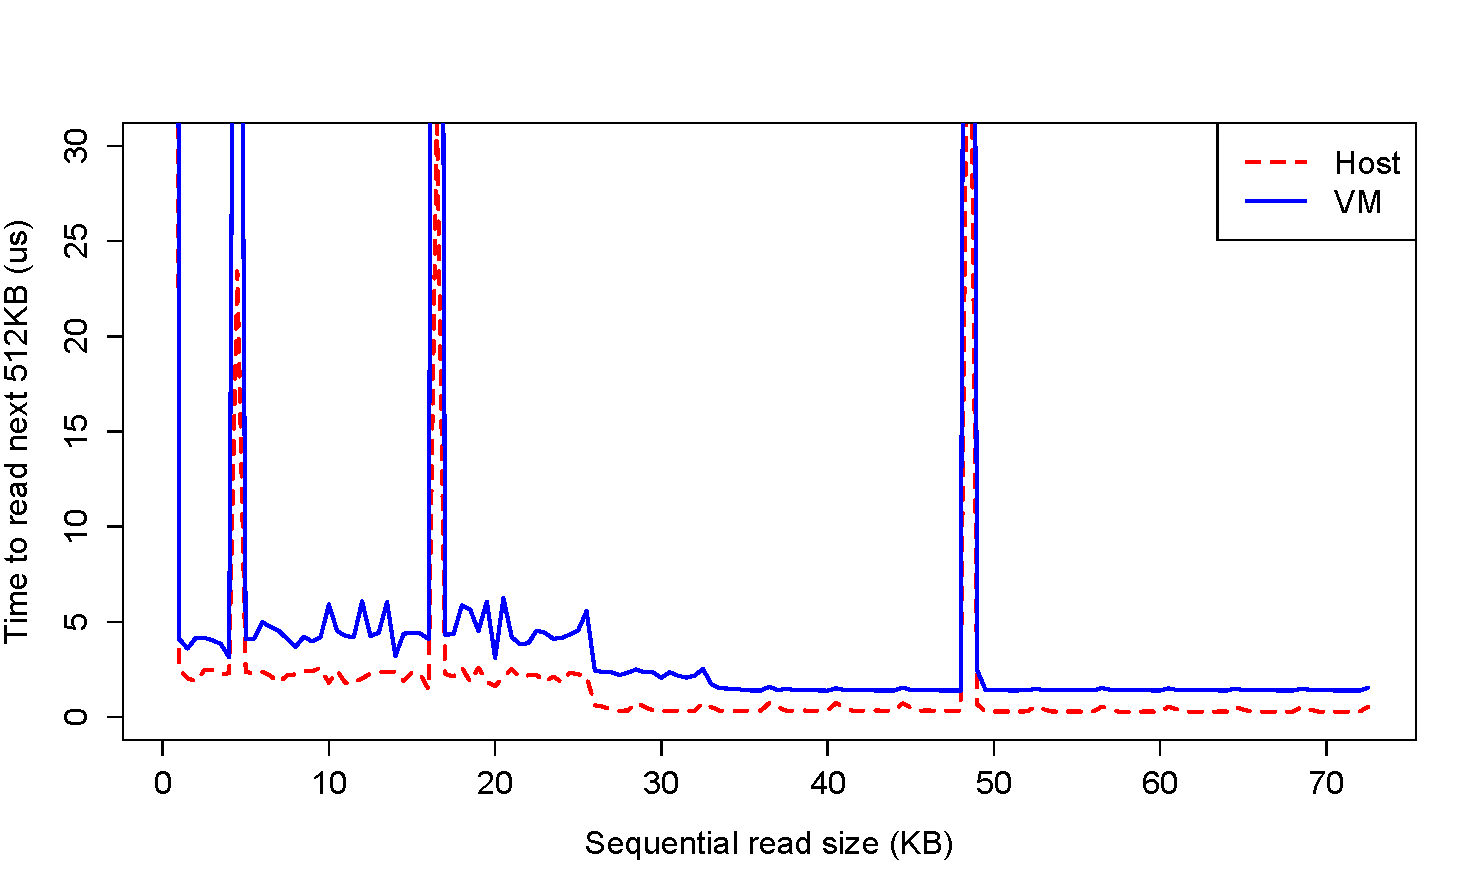
\includegraphics[width=\textwidth]{./figures/p2_small.pdf}
	\caption{A close up view of latency versus number of read bytes}
	\label{fig:p2_graph_small}
	\end{subfigure}
	\caption{Time to read 512KB blocks with respect to total number of KB read sequentially from a file}
\end{figure}

Since the latency is higher (due to trap into readahead) when either there is a page 
fault or if the application references the page indicated by the lookahead index,
we can find the prefetch size by performing sequential reads and determining
the sizes in which spikes occur. Typically the lookahead index refers to the first 
page of the readahead window. With this in mind, we wrote the code of 
Figure~\ref{fig:p2_code} to measure the prefetch size. In our code, we flush 
the cache before the initial read and measure the time to read READ\_SIZE number of
bytes at a time. We then wait 100ms to allow time for pages to be prefetched. This
eliminates false positives in the case where the read requests occur faster than
the data can be fetched from disk, resulting in a page fault.

Figure~\ref{fig:p2_graph_big} shows the read latency for a READ\_SIZE of 512B with
respect to the total number of bytes read. We see spikes for the host and VM at the
same places in the read sequence. We observe high latency for the initial read, and
then at increasing intervals of 4KB, 12KB, 32KB, and 64KB. After this the spikes 
occur at fixed intervals of 128KB. Thus, readahead behaves as we expect with a
window that grows until it reaches the maximum prefetch size. 
A closer inspection of the graph in Figure~\ref{fig:p2_graph_small} shows that the 
read latency is consistently greater than the latency on the host machine by a 
approximately 2$\mu$s. This suggests that the VM incurs some fixed overhead on 
reads from disk. This may be due to the hypervisor updating the VM shadow page 
table on a page fault.




